\lstinputlisting[language=bash,basicstyle=\small]{python_codes/fieldstone_47/keywords.ascii}

\begin{center}
Code at \url{https://github.com/cedrict/fieldstone/tree/master/python_codes/fieldstone_47}
\end{center}

\par\noindent\rule{\textwidth}{0.4pt}
%%%%%%%%%%%%%%%%%%%%%%%%%%%%%%%%%%%%%%%%%%%%%%%%%%%%%%%%%%%%%%%%%%%%%%%%%%%%%%%%%%%%%%%%%%%%

The domain is a unit square and the grid is composed of triangles but for simplicity these 
are obtained by splitting rectangles in two, as shown hereunder:

\begin{center}
\includegraphics[width=8cm]{python_codes/fieldstone_47/images/minigrid}\\
Not shown are the nodes for the bubbles in the middle of each triangle. 
\end{center}

This stone showcases the MINI element (see Section~\ref{MMM-pair:mini})
used to solve the analytical problem "Donea \& Huerta" (see Section~\ref{MMM-mms1}).
Out of convenience the pressure is set to zero at location $(x,y)=(1,1)$, so that the 
analytical solution is now $p(x,y)=x(1-x)$. 

As an experiment I have run convergence tests for two cases: using {\tt nqel=3},  
{\tt nqel=6} and {\tt nqel=7} quadrature points.
We find that the velocity and pressure errors convergence depends on this crucial parameter. 
For {\tt nqel=3} the velocity and pressure errors converge quadratically and linearly respectively
but for {\tt nqel=6,7} they converge as $h^2$ and $h^{1.5}$ respectively:

\begin{center}
\includegraphics[width=12cm]{python_codes/fieldstone_47/images/reg/errors}
\end{center}

It is worth noticing that although the element is stable, and the error converges
at a respectable rate, the pressure solution is not 'clean': as shown on the 
following figure, there is still some under/overshoot with respect to the analytical solution.

\begin{center}
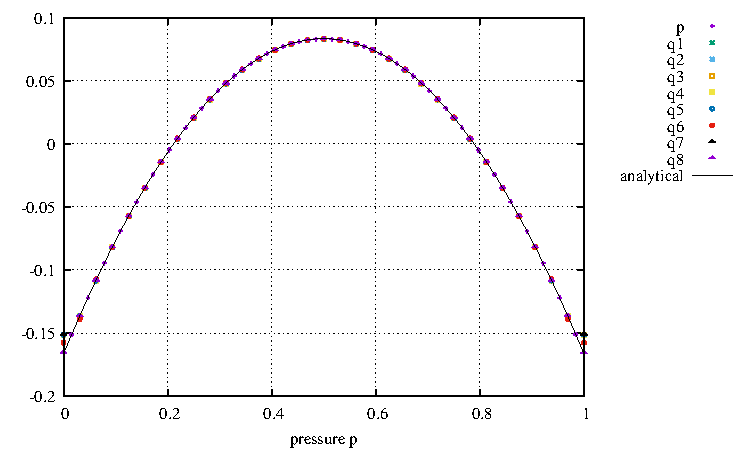
\includegraphics[width=8cm]{python_codes/fieldstone_47/images/reg/pressure.pdf}
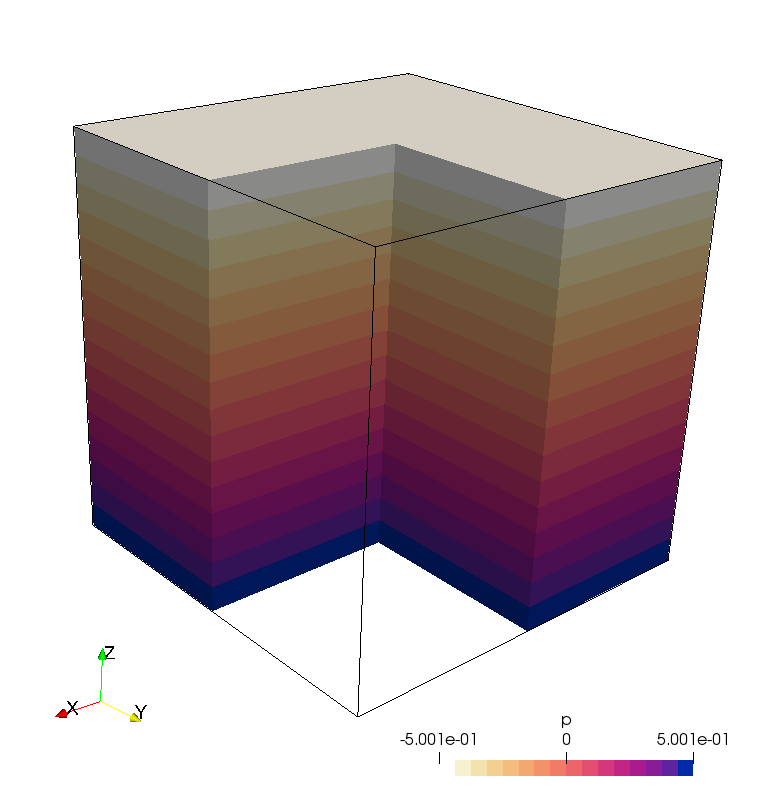
\includegraphics[width=6cm]{python_codes/fieldstone_47/images/rand/press}
\end{center}

Let us now explore the case where the nodes inside the domain are randomly perturbed, i.e. 
a random value  $(\delta_x,\delta_y)\in[-h_x/5,h_x/5]\times[-h_y/5,h_y/5]$ is added 
to their position (while preserving the position of the bubble as the barycenter of each triangle), 
as shown hereunder:

\begin{center}
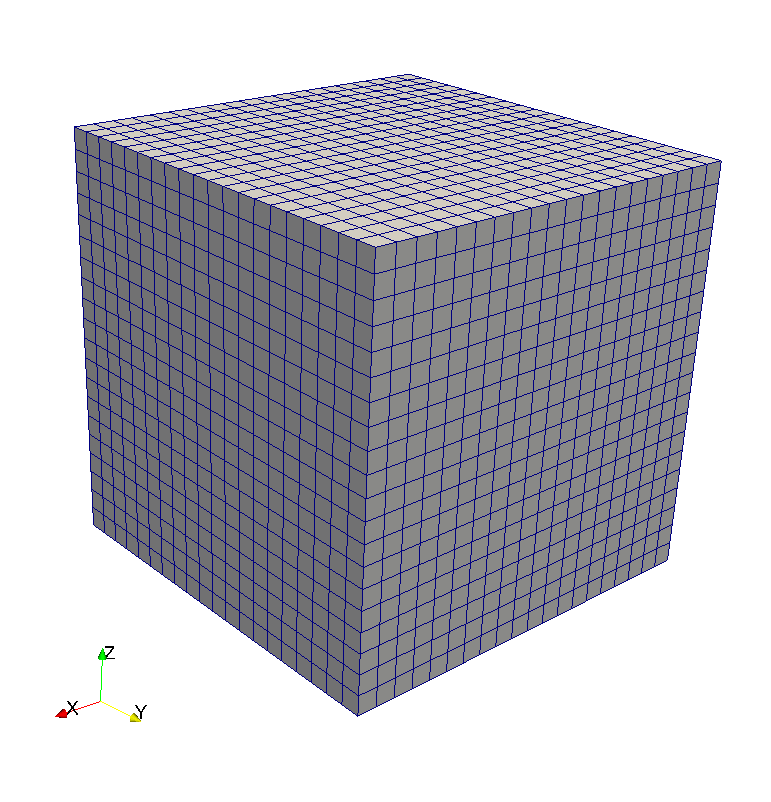
\includegraphics[width=7cm]{python_codes/fieldstone_47/images/rand/grid}
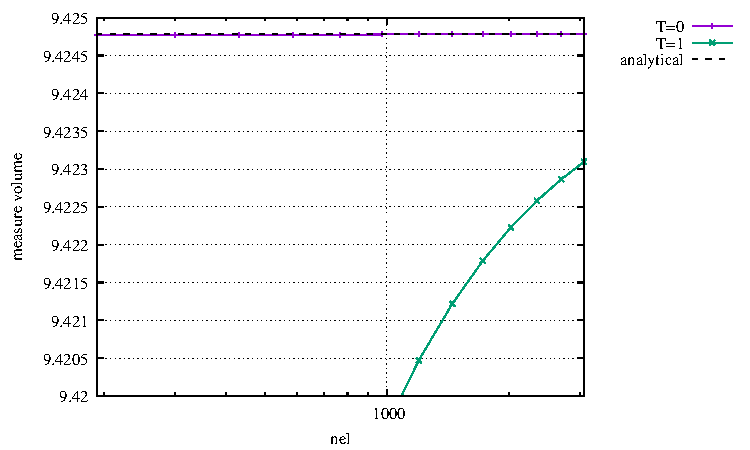
\includegraphics[width=7cm]{python_codes/fieldstone_47/images/rand/areas}
\end{center}
 
Looking again at the convergence rates of the errors, we see that the velocity errors 
are virtually unchanged but we observe that the pressure errors no more align on a
single line and that the rates are only maintained on average. 

\begin{center}
\includegraphics[width=12cm]{python_codes/fieldstone_47/images/rand/errors}
\end{center}

